%; whizzy paragraph -pdf xpdf -latex ./whizzypdfptex.sh
%; whizzy-paragraph "^\\\\begin{frame}\\|\\\\emtext"
% latex beamer presentation.
% platex, latex-beamer $B$G%3%s%Q%$%k$9$k$3$H$rA[Dj!#(B 

%     Tokyo Debian Meeting resources
%     Copyright (C) 2012 Junichi Uekawa

%     This program is free software; you can redistribute it and/or modify
%     it under the terms of the GNU General Public License as published by
%     the Free Software Foundation; either version 2 of the License, or
%     (at your option) any later version.

%     This program is distributed in the hope that it will be useful,
%     but WITHOUT ANY WARRANTY; without even the implied warreanty of
%     MERCHANTABILITY or FITNESS FOR A PARTICULAR PURPOSE.  See the
%     GNU General Public License for more details.

%     You should have received a copy of the GNU General Public License
%     along with this program; if not, write to the Free Software
%     Foundation, Inc., 51 Franklin St, Fifth Floor, Boston, MA  02110-1301 USA

\documentclass[cjk,dvipdfmx,12pt]{beamer}
\usetheme{Tokyo}
\usepackage{monthlypresentation}

%  preview (shell-command (concat "evince " (replace-regexp-in-string "tex$" "pdf"(buffer-file-name)) "&")) 
%  presentation (shell-command (concat "xpdf -fullscreen " (replace-regexp-in-string "tex$" "pdf"(buffer-file-name)) "&"))
%  presentation (shell-command (concat "evince " (replace-regexp-in-string "tex$" "pdf"(buffer-file-name)) "&"))

%http://www.naney.org/diki/dk/hyperref.html
%$BF|K\8l(BEUC$B7O4D6-$N;~(B
\AtBeginDvi{\special{pdf:tounicode EUC-UCS2}}
%$B%7%U%H(BJIS$B7O4D6-$N;~(B
%\AtBeginDvi{\special{pdf:tounicode 90ms-RKSJ-UCS2}}

\newenvironment{commandlinesmall}%
{\VerbatimEnvironment
  \begin{Sbox}\begin{minipage}{1.0\hsize}\begin{fontsize}{8}{8} \begin{BVerbatim}}%
{\end{BVerbatim}\end{fontsize}\end{minipage}\end{Sbox}
  \setlength{\fboxsep}{8pt}
% start on a new paragraph

\vspace{6pt}% skip before
\fcolorbox{dancerdarkblue}{dancerlightblue}{\TheSbox}

\vspace{6pt}% skip after
}
%end of commandlinesmall

\title{$BEl5~%(%j%"(BDebian$BJY6/2q(B\\Debian$B%Q%C%1!<%8%s%0F;>l(B}
\subtitle{$BBh(B130$B2s(B 2015$BG/(B9$B7nEY(B}
\author{$B4d>>(B $B?.MN(B}
\date{2015$BG/(B9$B7n(B12$BF|(B}
\logo{
\includegraphics[width=8cm]{image200607/openlogo-light.eps}}

\begin{document}

\begin{frame}
\titlepage{}
\end{frame}

\begin{frame}{$B@_1D=`Hw$K$46(NO$/$@$5$$!#(B}
$B2q>l@_1D$h$m$7$/$*$M$,$$$7$^$9!#(B
\end{frame}

\begin{frame}{Agenda}
\begin{itemize}
   \item $B:G6a$"$C$?(BDebian$B4XO"$N%$%Y%s%HJs9p(B
	 \begin{itemize}
	 \item $BBh(B129$B2s(B $BEl5~%(%j%"(BDebian$BJY6/2q(B
	 \item OSC 2015 Niigata
	 \end{itemize}
   \item $B%Q%C%1!<%8%s%0%A%e!<%H%j%"%k$r;H$C$?2r@b(B
   \item $B%Q%C%1!<%8%s%0F;>l(B
   \item $B:#8e$N%$%Y%s%H(B
   \item $B:#F|$N1c2q>l=j(B
  \end{itemize}
\end{frame}

\section{$B%$%Y%s%HJs9p(B}
\emtext{$B%$%Y%s%HJs9p(B}

\begin{frame}{$BBh(B129$B2sEl5~%(%j%"(BDebian$BJY6/2q(B}

\begin{itemize}
\item $B>l=j$O%9%/%&%'%"!&%(%K%C%/%9$5$s$N%;%_%J%k!<%`$r$*<Z$j$7$F$N3+:E$G$7$?!#(B
\item $B%;%_%J$OLnEg$5$s$K$h$k!V(BAPT1.1 $BD6!y5m$5$s%Q%o!<_ZNv(B!$B!W$HBj$7$?(B APT 1.1 $B$N2r@b$G$7$?!#(B
\item $B;D$j$N;~4V$G(Bhack time$B$r9T$$!"@.2LH/I=$r$7$^$7$?!#(B
\end{itemize} 
\end{frame}

\begin{frame}{OSC 2015 Niigata}

\begin{itemize}
\item 9/8 $B$K(B $B?73c$G(BOSC$B$,3+:E$5$l!"LnEg$5$s$H5HED$5$s$,$5$s$+$5$l$^$7$?!#(B\url{/http://www.ospn.jp/osc2015-niigata/}
\item $B%;%_%J$HE8<($r9T$$!"%;%_%J!<$OLnEg$5$s$K$h$k!V(BDebian update$B!W$HBj$7$?(B Debian 8.0 $B$N>R2p$,9T$o$l$^$7$?!#(B
\end{itemize} 

\end{frame}

\section{Debian $B%Q%C%1!<%8%s%0F;>l(B}
\emtext{Debian $B%Q%C%1!<%8%s%0F;>l(B}

\begin{frame}{$BK\F|$NN.$l(B}

\begin{itemize}
 \item $B8aA0$NIt(B
  \begin{itemize}
   \item $B%Q%C%1!<%8%s%0%A%e!<%H%j%"%k$r;H$C$?(B Debian $B%Q%C%1!<%8$N2r@b(B
   \item git buildpackage $B$N;H$$J}$r2r@b(B
  \end{itemize}
 \item $B$*Ck$4$O$s(B
 \item $B8a8e$NIt(B (13:00 -)
  \begin{itemize}
   \item $B%Q%C%1!<%8:n6H(B
   \item $B@.2LJs9p(B
  \end{itemize}
\end{itemize}

\end{frame}

\emtext{$B%Q%C%1!<%8%s%0%A%e!<%H%j%"%k(B}
\emtext{git buildpackage}

\begin{frame}

Debian $B%Q%C%1!<%8%s%0%A%e!<%H%j%"%k$G$"$^$j2r@b$5$l$F$$$J$$(B gbp (git
buildpackage) $B$N4pK\E*$J;H$$J}$K$D$$$F@bL@$9$k!#(B

\end{frame}

\begin{frame}{VCS $B$G4IM}$7$J$$>l9g(B}

\begin{center}
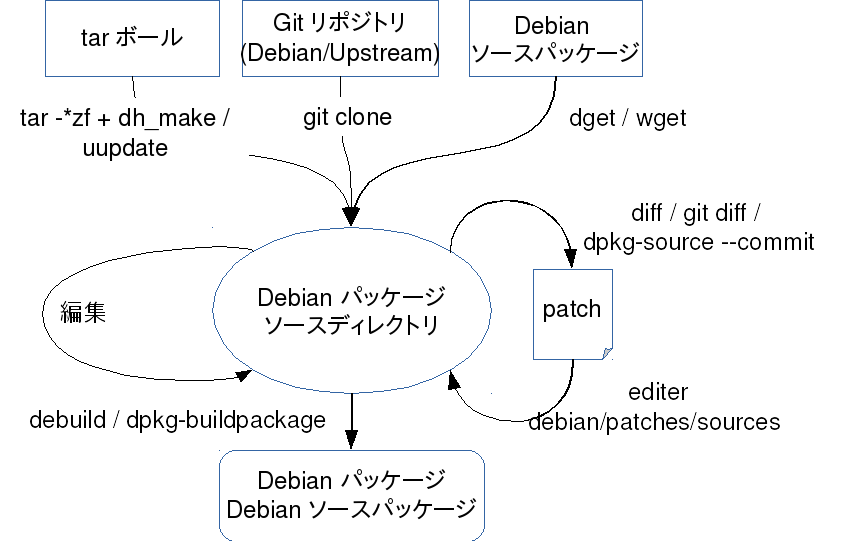
\includegraphics[width=0.8\hsize]{image201509/gbp-images0.png}
\end{center}

\end{frame}

\begin{frame}{VCS $B$G4IM}$9$k>l9g(B}
\begin{center}
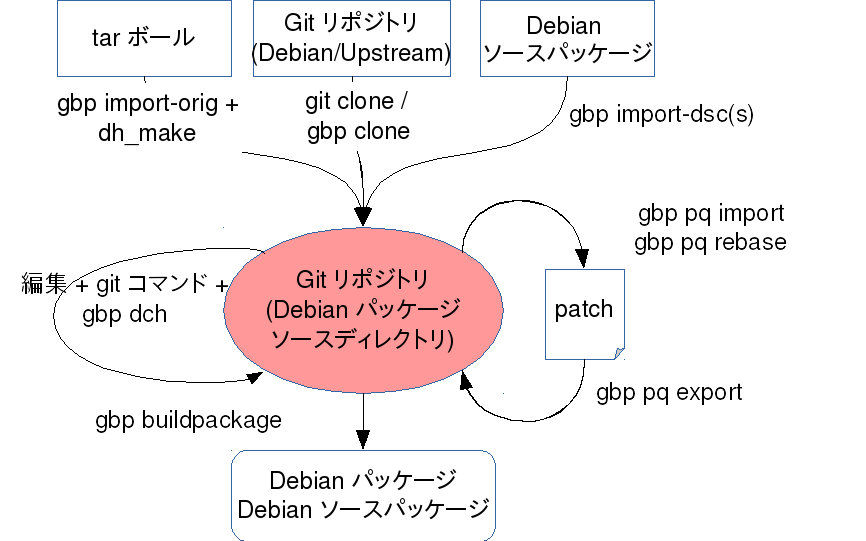
\includegraphics[width=0.8\hsize]{image201509/gbp-images1.png}
\end{center}
\end{frame}

\begin{frame}[containsverbatim]{Upstream $B$+$i(B tar $B%\!<%k$,%j%j!<%9$5$l$F$$$k>l9g(B}

Upstream $B$+$i(Btar$B%\!<%k$,%j%j!<%9$5$l$F$$$k>l9g!"(B
tar $B%\!<%k$r(BGit$B%j%]%8%H%j$K%3%_%C%H$7$?8e!"%Q%C%1!<%82=$r9T$&!#(B

\end{frame}

\begin{frame}[containsverbatim]
\begin{itemize}
\item tar $B%\!<%k$r%@%&%s%m!<%I$9$k(B

\begin{commandline}
$ wget package-name-0.0.1.tar.gz
\end{commandline}

\item Git$B%j%]%8%H%j$r:n@.$9$k(B

\begin{commandline}
$ git init package-name
$ cd package-name
\end{commandline}

$BI,MW$G$"$l$P(B git config $B$G(B Git $B$N@_Dj$rJQ99$9$k!#(B
\end{itemize}
\end{frame}

\begin{frame}[containsverbatim]
\begin{itemize}
\item tar $B%\!<%k$r;XDj$7$F!"%=!<%9%3!<%I$r(B Git $B$K%3%_%C%H$9$k(B

\begin{commandline}
$ gbp import-orig --pristine-tar \
	../package-name-0.0.1.tar.gz
$ git tag 
$ upstream/0.0.1
$ git branch
* master
  upstream
\end{commandline}
\end{itemize}
\end{frame}

\begin{frame}[containsverbatim]
\begin{itemize}
\item Upstream$B$N%3!<%I$r$O(B upstream $B%V%i%s%A$G4IM}$5$l!"F1;~$K%?%0$,@_(B
$BDj$5$l$k!#(B
\item pristine-tar $B%*%W%7%g%s$O%*%j%8%J%k$N(Btar$B%\!<%k$N:9J,$rJ]B8$9$k$?$a$N;EAH$_$rM-8z(B
$B$K$9$k!#(BUpstream$B$N%3!<%I$O(B upstream $B%V%i%s%A$G4IM}$5$l!"(BDebian $B%Q%C%1!<%8$r(B
$B:n@.$9$k$H$-$K!"$=$3$+$i(B orig.tar.gz $B%U%!%$%k$r:n@.$9$k!#$3$N;~$K:n@.$5$l$k%U%!%$%k(B
$B$,F1$8$b$N$K$J$i$J$$>l9g$,$"$k!#(BDebian $B$G$O(B
$B<h$j9~$s$@(B tat.gz $B%U%!%$%k$N%O%C%7%eCM$H(BDebian $B%=!<%9%Q%C%1!<%8$H$7$F%"%C%W%m!<%I$5$l$k(B
tar.gz $B%U%!%$%k$,F1$8$G$"$kI,MW$,$"$k$?$a!"K\%*%W%7%g%s$rMQ$$$F(B orig.tar.gz$B$H$N:9J,$r(B
$B%P%$%J%j%Q%C%A$H$7$FJ]B8$7!"(Borig.tar.gz$B$r9=C[$9$kEY$K:FE,MQ$9$k$3$H$G!"%O%C%7%eCM(B
$B$,F1$8(Borig.tar.gz$B$r:F9=C[$G$-$k$h$&$K$7$F$$$k!#(B
\end{itemize}
\end{frame}

\begin{frame}[containsverbatim]
\begin{itemize}
\item dh\_make $B$G(B debian $B%G%#%l%/%H%j$N?w7A$r:n@.$9$k(B 

\begin{commandline}
$ dh_make -p package-name_0.0.1
\end{commandline}

\item debian $B%G%#%l%/%H%jFb$r$$$m$$$mJQ99$9$k(B

\begin{commandline}
$ $B$$$m$$$m=$@5(B
$ git add debian
$ git commit
\end{commandline}
\end{itemize}
\end{frame}

\begin{frame}[containsverbatim]
\begin{itemize}
\item $B%Q%C%1!<%82=:n6H$,$G$-$?$i(B $B%Q%C%1!<%8$r9=C[$9$k(B

\begin{commandline}
$ gbp buildpackage --git-pristine-tar
\end{commandline}

\item piuparts $B$J$I$G%$%s%9%H!<%k!"%"%s%$%s%9%H!<%k$N%F%9%H(B

\item $B:G8e$K%/%j!<%s$J4D6-$G%S%k%I%F%9%H(B

\begin{commandline}
$ git-pbuilder
or
$ gbp buildpackage --git-pbuiler --git-pristine-tar
\end{commandline}
\end{itemize}
\end{frame}

\begin{frame}[containsverbatim]
\begin{itemize}
\item $B%?%0$r@_Dj$7$F(B $B%j%b!<%H%j%]%8%H%j$K%W%C%7%e$9$k(B

\begin{commandline}
$ gbp buildpackage --git-tag-only
$ git push
\end{commandline}

\end{itemize}
\end{frame}

\begin{frame}{upstream $B$K99?7$,$"$C$?>l9g(B}

\end{frame}

\begin{frame}[containsverbatim]
\begin{itemize}
\item upstream $B$N(Btar $B%\!<%k$r<hF@$9$k(B

\begin{commandline}
$ wget package-name-0.0.2.tar.gz
\end{commandline}

\item tar $B%\!<%k$r;XDj$7$F%j%]%8%H%j$K%=!<%9%3!<%I$r%3%_%C%H$9$k(B

\begin{commandline}
$ gbp import-orig --pristine-tar \
		../package-name-0.0.2.tar.gz
\end{commandline}

\texttt{--uscan} $B%*%W%7%g%s$G%@%&%s%m!<%I(B $\rightarrow$ $B%3%_%C%H$,0lEY$K$G$-$k!#(B
$B$^$?!"%=!<%9%3!<%I$O<+F0E*$K%^!<%8$5$l$^$9!#%^!<%8$7$?$/$J$$>l9g$O(B
\texttt{--no-merge} $B$r;XDj$7$F<B9T$9$k!#(B
\end{itemize}
\end{frame}

\begin{frame}[containsverbatim]
\begin{itemize}
\item debian/changelog $B$r=$@5(B

\begin{commandline}
$ dch -i
or
$ gbp dch 
\end{commandline}

\item $B%Q%C%1!<%8$r%S%k%I(B

\begin{commandline}
$ gbp buildpackage --git-pristine-tar \
		--git-pristine-tar-commit
\end{commandline}

\end{itemize}

\end{frame}

% -------------------------------------------------

\begin{frame}[containsverbatim]{Upstream $B$,(B Git $B$G4IM}$5$l$F$$$k>l9g(B}

\begin{itemize}
\item  Upstream $B$G$O(B tar $B%\!<%k$G%j%j!<%9$5$l$:!"(BGit$B$N%?%0$N$_$G%j%j!<%9$5$l$k>l9g(B
$B$b$"$k!#(B
\item Github $B$G3+H/$5$l$F$$$k%W%m%8%'%/%H$,NI$$Nc!#(B
\item $B$3$N$h$&$J>l9g$O(B $B%j%]%8%H%j$r%/%m!<%s$7$?8e!"(BDebian$BFH<+$N%V%i%s%A%k!<%k$rMQ$$$F(B
$B%=!<%9%Q%C%1!<%8$N4IM}$r9T$&!#(B
\end{itemize}

\end{frame}

\begin{frame}[containsverbatim]
\begin{itemize}

\item $B%j%]%8%H%j$r%/%m!<%s$7!":n@.$5$l$?%G%#%l%/%H%j$K0\F0$9$k(B

\begin{commandline}
$ git clone git://example.org/git/package-name.git
$ cd package-name
\end{commandline}
\end{itemize}
\end{frame}

\begin{frame}[containsverbatim]
\begin{itemize}
\item $B%Y!<%9$K$7$?$$%P!<%8%g%s$N%3!<%I$r%A%'%C%/%"%&%H$9$k(B

\begin{commandline}
$ git reset --hard 0.0.1
\end{commandline}
\end{itemize}
\end{frame}

\begin{frame}[containsverbatim]
\begin{itemize}
\item $B%?%0$r@_Dj$9$k(B

\begin{commandline}
$ git tag upstream/0.0.1
\end{commandline}

upstream $B%M!<%`%9%Z!<%9$O(B gbp $B%G%U%)%k%H;2>H@h!#(BUpstream$B$N%?%0$r;H$$$?$$>l9g(B
$B$dFH<+$N%M!<%`%9%Z!<%9$r;H$$$?$$>l9g$O(B gbp $B$N(B upstream-tag $B$,MxMQ$G$-$^$9!#(B

\begin{commandline}
[git-buildpackage]
upstream-tag = v%(version)s
\end{commandline}
\end{itemize}
\end{frame}

\begin{frame}[containsverbatim]
\begin{itemize}
\item dh\_make $B$G(B debian $B%G%#%l%/%H%j$N?w7A$r:n@.$9$k(B

\begin{commandline}
$ dh_make -p package-name_0.0.1
\end{commandline}
\end{itemize}
\end{frame}

\begin{frame}[containsverbatim]
\begin{itemize}
\item debian $B%G%#%l%/%H%jFb$r$$$m$$$mJQ99$9$k(B

\begin{commandline}
$ $B$$$m$$$m=$@5(B
$ git add debian
$ git commit
\end{commandline}
\end{itemize}
\end{frame}

\begin{frame}[containsverbatim]
\begin{itemize}
\item $B%Q%C%1!<%82=:n6H$,$G$-$?$i(B $B%Q%C%1!<%8$r9=C[$9$k(B

\begin{commandline}
$ gbp buildpackage --git-pristine-tar \
		--git-pristine-tar-commit
\end{commandline}

tar $B%\!<%k$r;H$&>l9g$H0[$J$k$N$O(B\texttt{--git-pristine-tar-commit} $B%*%W%7%g%s(B
$B$r;XDj$9$k$3$H!#$3$N%*%W%7%g%s$r;XDj$9$k$3$H$K$h$C$F%?%0$+$i(B orig.tar.gz $B$r@8@.(B
$B$9$k!#(B
\end{itemize}
\end{frame}

\begin{frame}[containsverbatim]
\begin{itemize}
\item piuparts $B$J$I$G%$%s%9%H!<%k!"%"%s%$%s%9%H!<%k$N%F%9%H(B

\item $B:G8e$K%/%j!<%s$J4D6-$G%S%k%I%F%9%H(B

\begin{commandline}
$ git-pbuilder
or
$ gbp buildpackage --git-pbuilder
\end{commandline}
\end{itemize}
\end{frame}

\begin{frame}[containsverbatim]
\begin{itemize}
\item $B%?%0$r@_Dj$7$F(B $B%j%b!<%H%j%]%8%H%j$K%W%C%7%e$9$k(B

\begin{commandline}
$ gbp buildpackage --git-tag-only
$ git push
\end{commandline}

\end{itemize}
\end{frame}

\begin{frame}{upstream $B$K99?7$,$"$C$?>l9g(B}

\end{frame}

\begin{frame}[containsverbatim]
\begin{itemize}
\item upstream $B$N%j%]%8%H%j>pJs$r<hF@$9$k(B

\begin{commandline}
$ git remote update
\end{commandline}
\end{itemize}
\end{frame}

\begin{frame}[containsverbatim]
\begin{itemize}
\item $BJQ99$r%^!<%8(B

\begin{commandline}
$ git tag upstream/0.0.2 0.0.2
$ git merge upstream/0.0.2
\end{commandline}
\end{itemize}
\end{frame}

\begin{frame}[containsverbatim]
\begin{itemize}
\item debian/changelog $B$r=$@5(B

\begin{commandline}
$ dch -i
or
$ gbp dch
\end{commandline}
\end{itemize}
\end{frame}

\begin{frame}[containsverbatim]
\begin{itemize}
\item $B%Q%C%1!<%8$r%S%k%I(B

\begin{commandline}
$ gbp buildpackage --git-pristine-tar\
		--git-pristine-tar-commit
\end{commandline}

\end{itemize}
\end{frame}

\begin{frame}{$B%"%C%W%9%H%j!<%`$N%=!<%9%3!<%IJQ99(B}

\begin{enumerate}
\item gbp pq import
\item Upstream $B%=!<%9%3!<%I$N=$@5(B
\item git commit
\item gbp pq export
\item git commit
\end{enumerate}

\end{frame}

\begin{frame}

\begin{center}
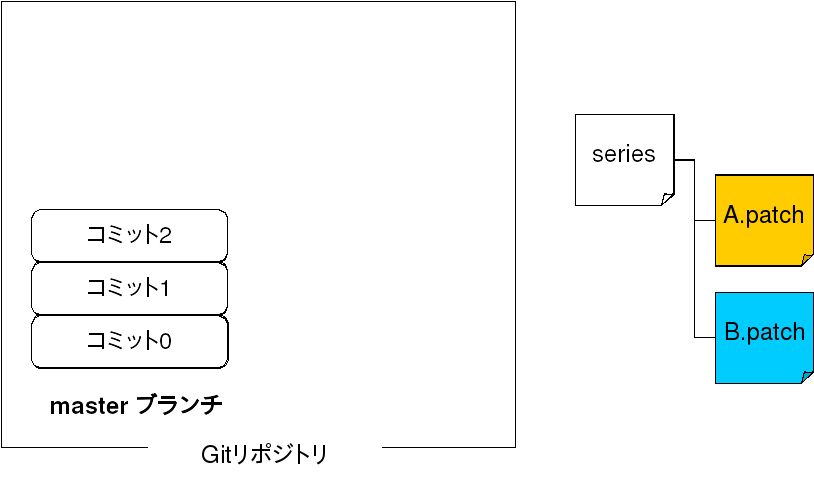
\includegraphics[width=0.8\hsize]{image201509/gbp-pq0.png}
\end{center}

\end{frame}

\begin{frame}{gbp pq import}

  \begin{enumerate}
   \item HEAD $B$r(Bpatch-queue/master $B%V%i%s%A$H$7$F%A%'%C%/%"%&%H(B
   \item debian/patches/series $B$K$"$k%Q%C%A$r%3%_%C%H(B
  \end{enumerate}

\begin{center}
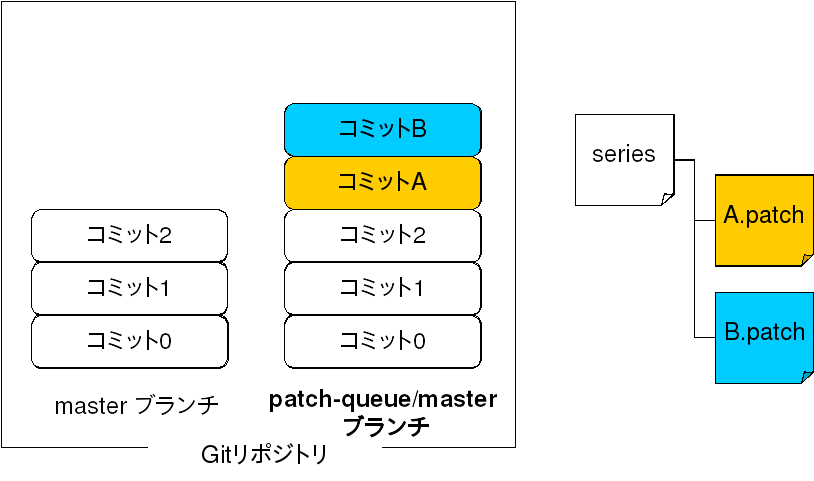
\includegraphics[width=0.8\hsize]{image201509/gbp-pq1.png}
\end{center}

\end{frame}

\begin{frame}{$B=$@5(B \& git commit}

  \begin{enumerate}
   \item Upstream $B%=!<%9%3!<%I$N=$@5(B
   \item git commit
  \end{enumerate}

\begin{center}
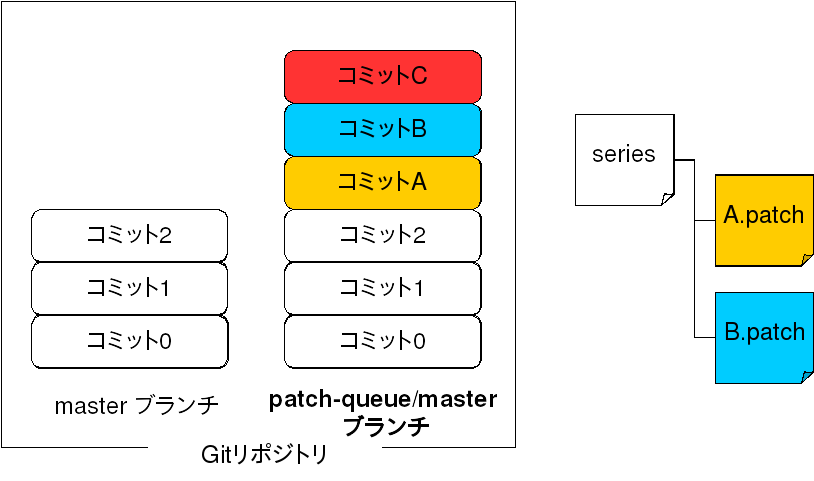
\includegraphics[width=0.8\hsize]{image201509/gbp-pq2.png}
\end{center}

\end{frame}

\begin{frame}{gbp pq export}
  \begin{enumerate}
   \item patch-queue/master $B$H(B master $B%V%i%s%A$N:9J,$r%Q%C%A$H$7$F(B debian/patches $B$K=PNO(B
   \item debian/patches/series $B$r99?7(B
   \item master $B%V%i%s%A$r%A%'%C%/%"%&%H(B
  \end{enumerate}

\begin{center}
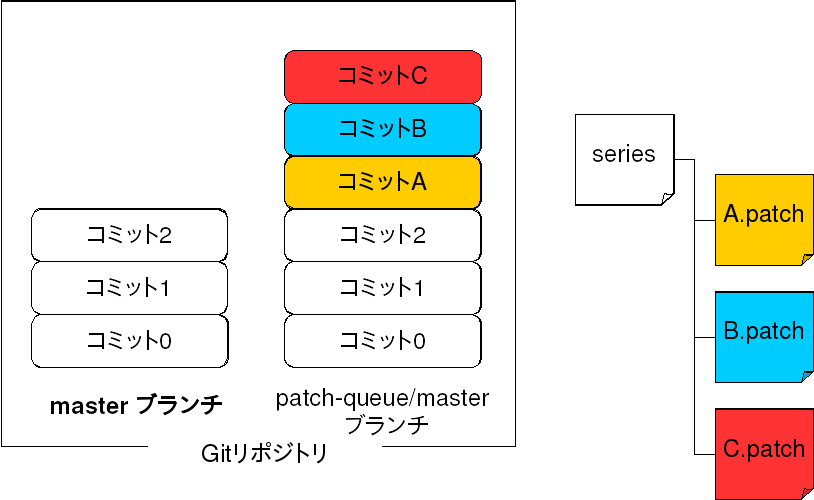
\includegraphics[width=0.8\hsize]{image201509/gbp-pq3.png}
\end{center}
  
  
\end{frame}

\begin{frame}{git commit}
  \begin{enumerate}
   \item $B%Q%C%A99?7$r%j%]%8%H%j$K%3%_%C%H(B
  \end{enumerate}

\begin{center}
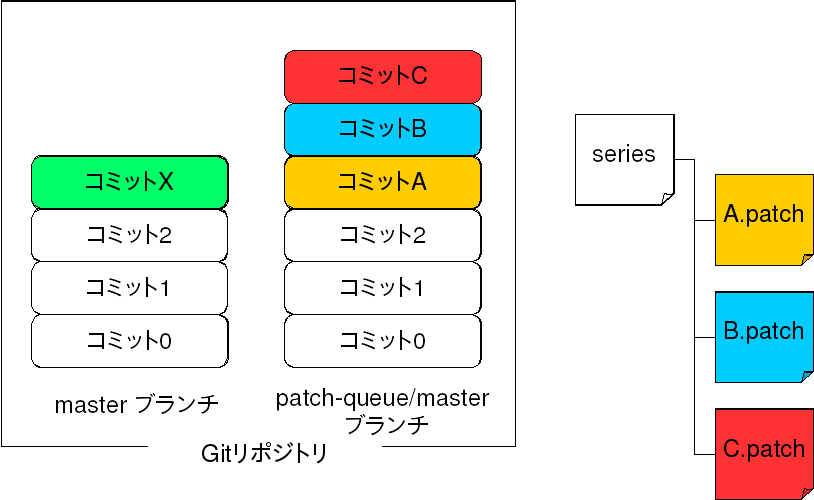
\includegraphics[width=0.8\hsize]{image201509/gbp-pq4.png}
\end{center}
\end{frame}

\begin{frame}{$B$^$H$a(B}

\begin{itemize}
\item gbp (git buildpackage)$B$O%G%U%!%/%H%9%?%s%@!<%H(B
\item gbp import-* $B$G%j%]%8%H%j<h$j9~$_(B
  
  \texttt{--pristine-tar} $B$rK:$l$:$K(B
\item gbp dch $B$G(B debian/changelog $B$r99?7(B
\item gbp buildpackage $B$G%Q%C%1!<%8%S%k%I(B
\item gbp pq $B$G%Q%C%AA`:n(B
\end{itemize}


\end{frame}

\emtext{$B%Q%C%1!<%8:n6H(B}
\emtext{$B@.2LJs9p(B}

\section{$B:#8e$N%$%Y%s%H(B}
\emtext{$B:#8e$N%$%Y%s%H(B}
\begin{frame}{$B:#8e$N%$%Y%s%H(B}
\begin{itemize}
 \item $B4X@>%(%j%"(BDebian$BJY6/2q(B
 \item 10/24($BEZ(B)$B!"(B10/25($BF|(B) OSC 2015 Tokyo Fall$B$G%;%_%J!u%V!<%9(B\\
\url{http://www.ospn.jp/osc2015-fall/}
\end{itemize}
\end{frame}

\section{$B:#F|$N1c2q>l=j(B}
\emtext{$B:#F|$N1c2q>l=j(B}
\begin{frame}{$B:#F|$N1c2q>l=j(B}
$BL$Dj(B
\end{frame}

\end{document}

;;; Local Variables: ***
;;; outline-regexp: "\\([ 	]*\\\\\\(documentstyle\\|documentclass\\|emtext\\|section\\|begin{frame}\\)\\*?[ 	]*[[{]\\|[]+\\)" ***
;;; End: ***
